\section{Numerical Examples}
We perform $h$- and $p$- convergence studies on ground state energy ($E_0$) computation for 
carbon (C) atom which has $6$ electrons. As per the {\bf NIST} standard the $E_0$ for C is $(E_0)_{\textrm{exact}} = -37.425749$ Hartree. 
To this end, we consider the domain $[\texttt{rmin} \, \, \texttt{rmax}] = [0 \, \, 10]$ a.u., meshed with \texttt{numel} equi-spaced 
elements.
%
\subsection{$p$-Convergence} 
For a fixed \texttt{numel} the element order $p$ is varied as $1, 2, \ldots, 10$ . For each of these $p$, $E_0$ value is 
reported. Increasing $p$ increases the number of DOF and hence, ideally we should converge to the $(E_0)_{\textrm{exact}}$. 
Subsequently, we also consider $\texttt{numel} = 10, 20$, and $40$. This set of numerical experiments are performed using 
the script \texttt{testpconvergence.m}.
%
\begin{figure}[h!]
	\centering
	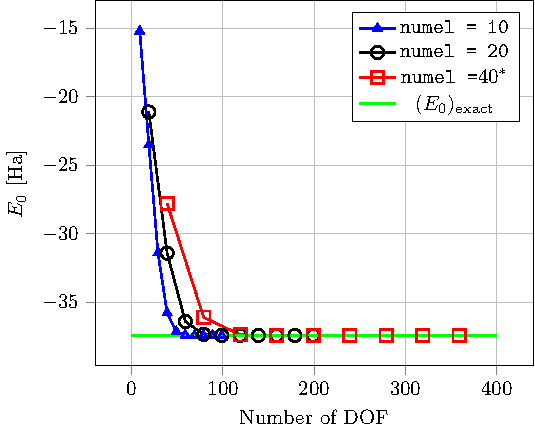
\includegraphics[width=1\textwidth]{pconv.pdf}
	\caption{p-Convergence ($\ast$ \texttt{eigs} failed for $\texttt{numel} = 40$ with $p = 10$)}
\end{figure}
%
\subsection{$h$-Convergence}
For a fixed element order $p$ the element order \texttt{numel} is varied as $5, 10, 20,$ and $40$. 
For each of these \texttt{numel}, $E_0$ value is reported. Increasing \texttt{numel} once again increases the 
number of DOF and hence, ideally we should converge to the $(E_0)_{\textrm{exact}}$. 
Cases with $p = 2, 4$, and $8$ are considered. This set of numerical experiments are performed using  
the script \texttt{testhconvergence.m}.
\begin{figure}[h!]
	\centering
	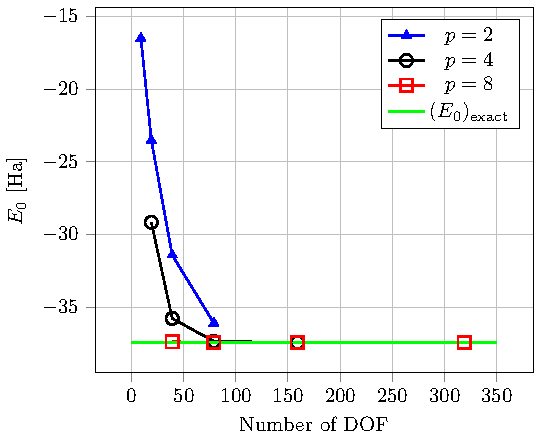
\includegraphics[width=1\textwidth]{hconv.pdf}
	\caption{h-Convergence}
\end{figure}
